\chapter{Related Work}
\label{chap:RelatedWork}

\section{The U-Net architecture}

The article \emph{U-Net: Convolutional Networks for Biomedical Image Segmentation} (\cite{UNet}) introduces a fully-convolutional neural network, that is surprisingly good at performing image segmentation. The article uses the architecture for semantic segmentation and instance segmentation of various biomedical images.

\begin{figure}[ht]
    \centering
    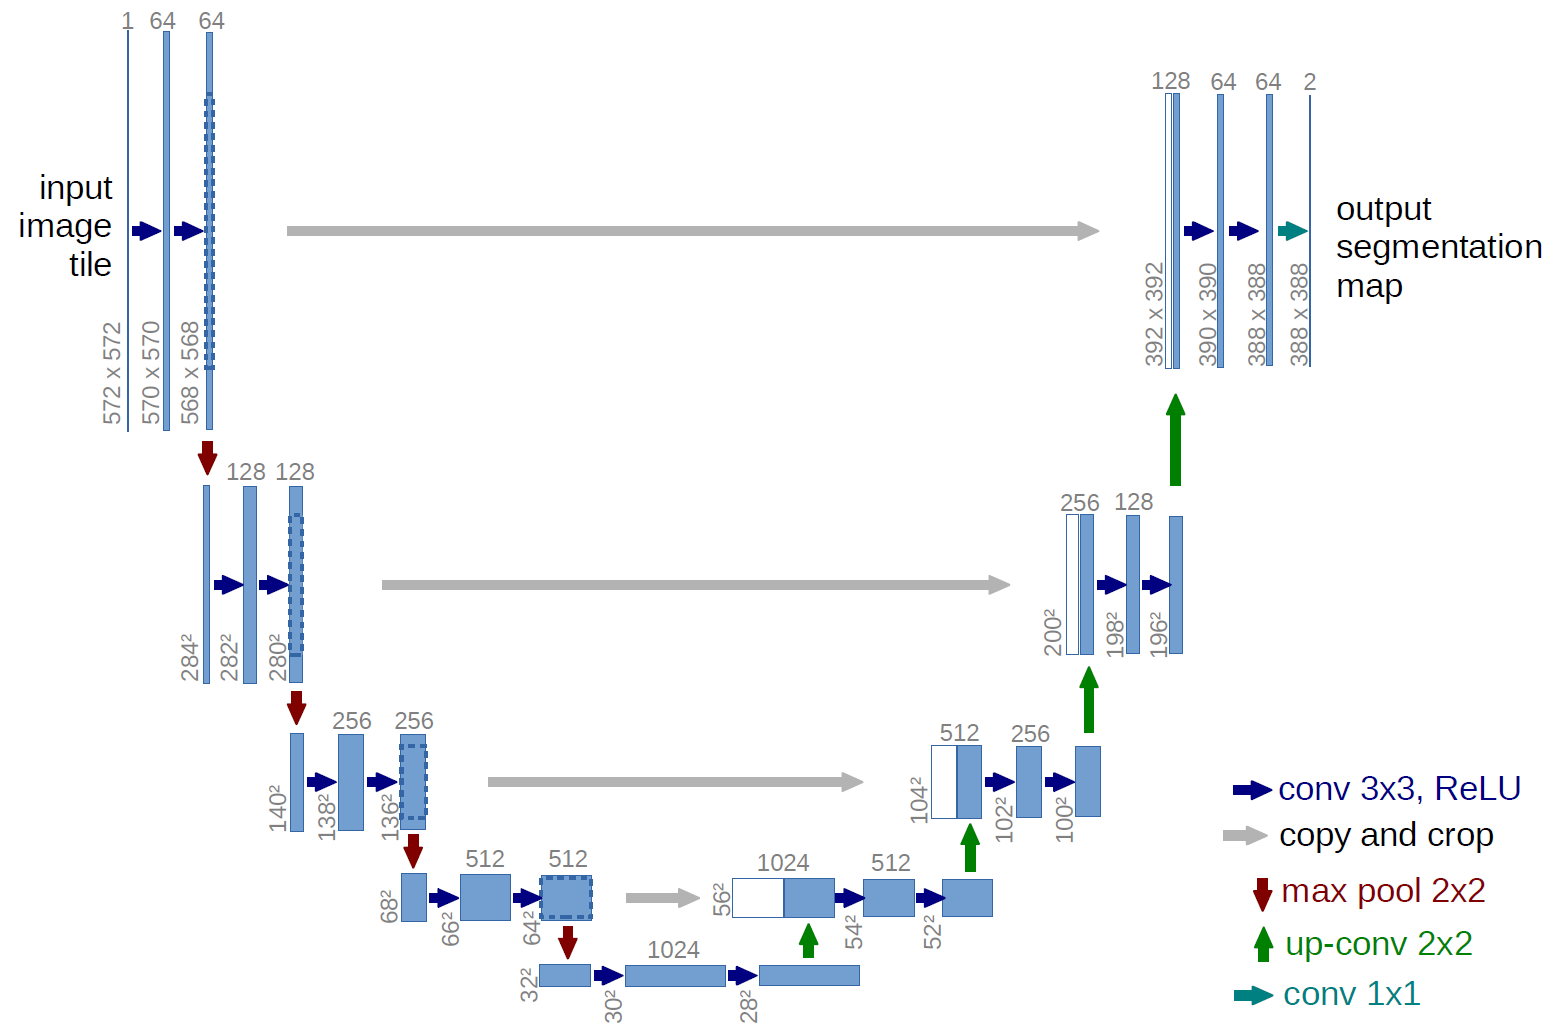
\includegraphics[width=145mm]{../img/u-net-architecture.png}
    \caption{The U-Net architecture with a contracting path and an expansive path. The image is taken from \cite{UNet}.}
    \label{fig:UNetArchitecture}
\end{figure}

The authors describe the left part of the network as the contracting path. It follows the typical layout of a convolutional network. The right part is called the expansive path. It is built as an inverse to the contractive part. The combination of a contraction with an expansion causes the network to first gather context information around each point of the image and then spread it back out to inform the segmentation process. The two halves are connected using skip-connections so that the expansive path also has accurate local information. Since the architecture resembles an autoencoder, we refer to the two halves of the network as an encoder and a decoder.


\section{Music object detection}

TODO: U-Net in music recognition (\cite{DorferEtAl}, \cite{HajicEtAl}) and its superiority in comparison to other CNN models (\cite{PachaBaseline}).

% = unet i OMR
% dorfer, hajič, pacha comparison


\section{Generative semi-supervised learning}

TODO: All the unsupervised, semi-supervised, clustering and disentagnling features of adversarial autoencoders (\cite{AdversarialAutoencoders}). Pioneered by smisup VAE (\cite{KingmaSslVae}).

% adversarial autoencoders
% which has been pioneered by M1+M2 VAE
